\setAuthor{Hans Daniel Kaimre}
\setRound{piirkonnavoor}
\setYear{2024}
\setNumber{G 3}
\setDifficulty{3}
\setTopic{TODO}

\prob{Valgusdioodid}
\begin{wrapfigure}{r}{0.5\textwidth}
  \vspace{-30pt}
  \begin{center}
  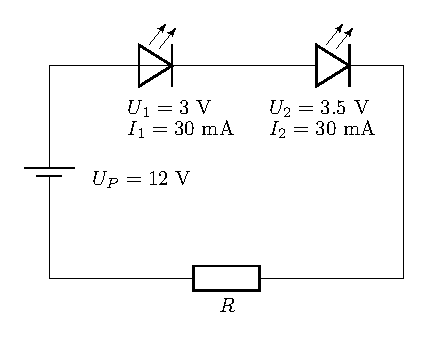
\includegraphics[scale=0.8]{2024-v2g-03-yl.pdf}
  \vspace{-20pt}
  \end{center}
\end{wrapfigure}

Mari koostas patareist ning kahest valgusdioodist (LEDist) vooluringi (vt joonist), kuid vooluahela kokkuühendamisel valgusdioodid põlesid läbi ning purunesid. Mari küsis isalt nõu, kes soovitas lisada vooluringi üks takisti. Aidake Maril välja mõelda, kui suure väärtusega takisti ja kuidas peaks ta skeemi lisama, et valgusdioodid töötaks normaaltingimustel. Joonistage uus vooluahel ning arvutage sobiva takisti väärtus. Patarei klemmipinge $U=\SI{12}{\V}$, valgusdioodide nimipinged on vastavalt $U_1=\SI{3}{V}$ ja $U_2=\SI{3.5}{V}$ ning optimaalne voolutugevus normaaltingimustel töötamisel $I_1=I_2=\SI{30}{\milli\A}$.


\hint

\solu
Kuivõrd LEDide nominaalne voolutugevus on võrdne, on mõistlik need ühendada omavahel jadamisi, nii nagu Mari seda tegi. Pingelang üle LEDide normaaltingimustel on $U_1+U_2=\SI{3}{\V}+\SI{3.5}{\V}=\SI{6.5}{\V}$, mis on tunduvalt vähem kui patarei klemmipinge $U=\SI{12}{V}$. Järelikult tuleb vooluringi ühendada LEDidega jadamisi takisti, millel pingelang oleks $U_R=U-U_1-U_2=\SI{12}{\V}-\SI{6.5}{\V}=\SI{5.5}{\V}$. Takisti väärtuse saame leida lihtsalt Ohmi seadusest, kuna takistit läbiv voolutugevus peab olema võrdne LEDe läbiva voolutugevusega: $R=U_R/I_1=\SI{5.5}{\V}/\SI{30}{\milli\A}=\SI{183}{\ohm}$.

\begin{figure}[h]
    \centering
    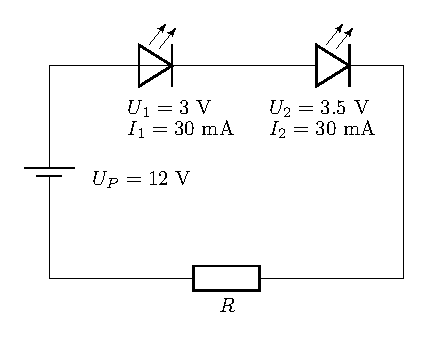
\includegraphics[width=0.5\linewidth]{2024-v2g-03-sol.pdf}
\end{figure}
\probend